\documentclass[mdthm]{scrartcl}
\usepackage[sexy]{evan}
\usepackage{hyperref}
\usepackage{ulem}
\usepackage{graphicx} % Required for inserting images
\usepackage{enumitem}
\usepackage{mathtools}
 
\title{User Manual}
\author{MidnightRaven12}
\date{April 2025}
\begin{document}
    \maketitle

    \begin{flushright}
        \begin{minipage}{0.3\textwidth}
            \footnotesize
            Given $n$ lines of code, you review it $O(\sqrt{n})$ times \\
            \noindent\rule{0.3\textwidth}{0.4pt} \\ % Horizontal line
            - Anonymous
        \end{minipage}
    \end{flushright}

    \tableofcontents


\section{Introduction}
  
Welcome to my project! 

\subsection{What is Whack-A-Mole for?}

Aim training is one of the most important skills that needs to developed in this country. More than the economic crises, and all of the political turmoil. Therefore, we have created Whack-A-Mole in order to address these concerns.

Bad aim can lead to a lot of psychological impacts, and can hinder a child’s social life. Ever since the 1980s when video games were invented, there was a higher demand for good aim. Nowadays, the modern lifestyle is to go back home and then to game. 

And for many children, not having good aim means that they get left out. An estimated 1 in 3 children will be left out. Additionally an estimated 65\% of statistics will be made up by 2040, (and more as we speak), as the Clicker Team, we will provide a solid product on training aim. 

\subsection{Mechanics}

It's just a basic game where you can, you know, whack some moles. You click on flashing red and yellow lights in order to gain points. Conversely, if you press on Grey Circles, you lose points and lives. There's also powerups, and stuff like that. So, really, just a basic minimalist game that people will play and just aim train on. It's minimalistic design can help ensure your child's concentration. 

\subsection{Basic Usage}

First, either use git clone, or just copy and paste the entire repository. 
If you want to run the game, please use the 'scripts/run.ps1' script in order to run the game. (If you want to compile the game, please use the script that is named 'compile', and use 'compile.sh' for Linux Systems.)   (cd scripts, and then ./compile.ps1 or ./compile.sh)

This compile script will compile all of your scripts into the (OUTPUT\_DIR Directory.) To add more, simply follow the pattern spelled out in the (javacCmd). 

It will output in the final\_project folder! 
\pagebreak


\section{Technical Stuff}

Here are the more technical things in the program. 

\subsection{Classes}

Those two important classes are the WhackAMoleGame.class and the Hole.class with the corresponding UML diagram here. 

\begin{figure}[h]  % 'h' specifies placement "here"
    \centering
    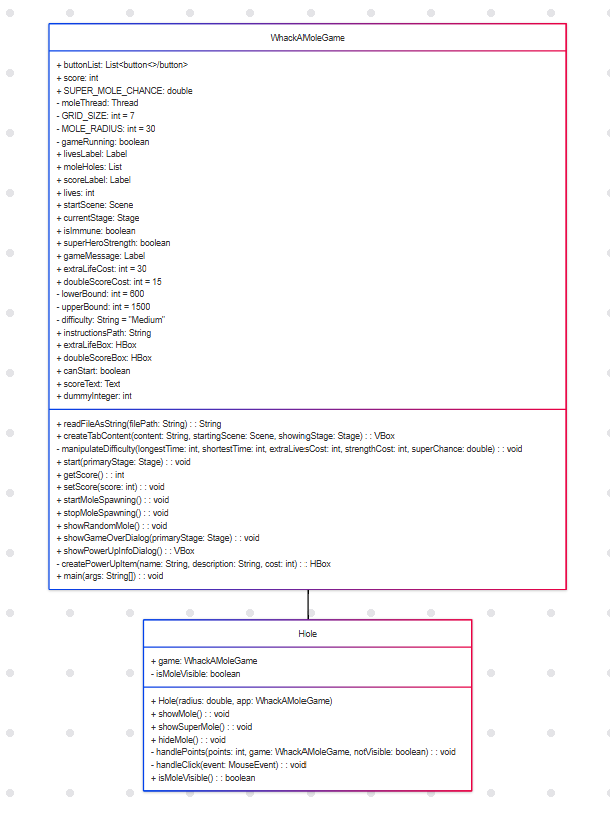
\includegraphics[width=0.8\textwidth]{../images/umlclassdiagram.png}
    \caption{Class Diagram}
    \label{fig:myimage}
\end{figure}

\pagebreak

In particular, the two most important methods are: start, (which starts the game), and startMoleSpawning. Those code snippets are: 

\begin{figure}[h]
    \centering
    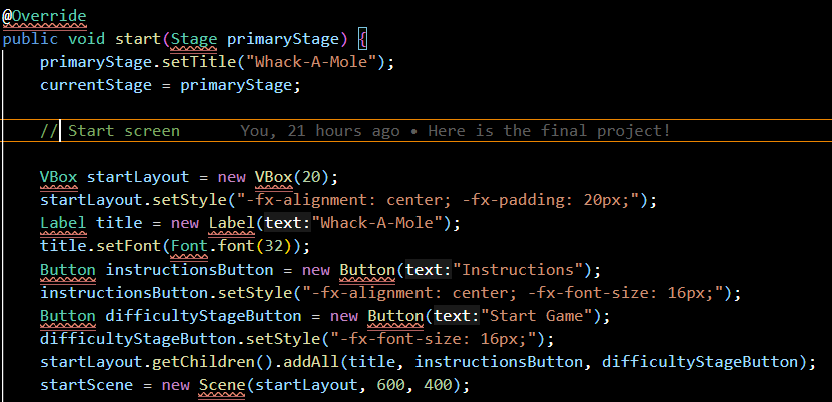
\includegraphics[width=0.8\textwidth]{../images/start.png}
    \caption{Start Method}
    \label{fig:myimage}
\end{figure}

and: 

\begin{figure}[h]
    \centering
    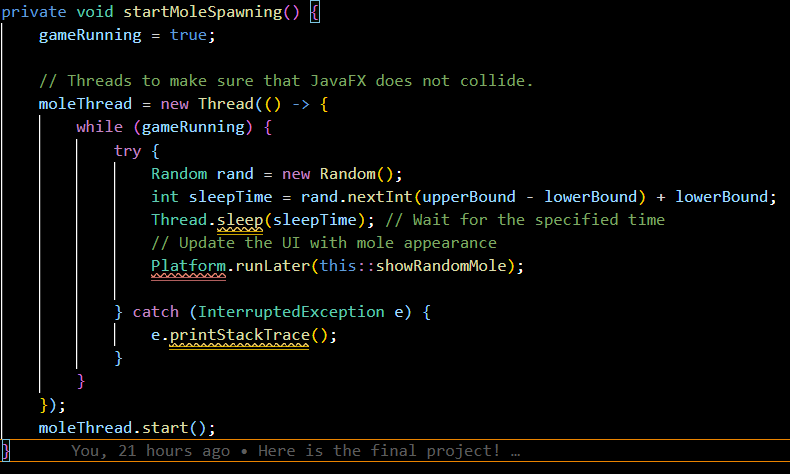
\includegraphics[width=0.8\textwidth]{../images/startMoleSpawning.png}
    \caption{Start Mole Method}
    \label{fig:myimage}
\end{figure}


The idea of startMoleSpawning is basically just, to start moles, as well as the start scene. Lastly, we also have: 

\begin{figure}[b]
    \centering
    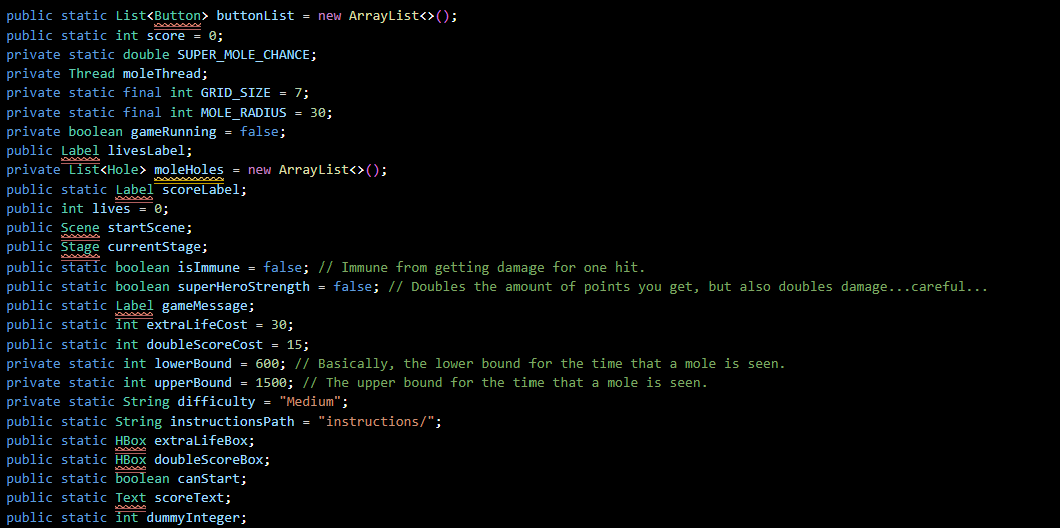
\includegraphics[width=0.8\textwidth]{../images/config.png}
    \caption{Config Values}
    \label{fig:myimage}
\end{figure}

These are variables to change how you play the game.

\subsection{Game Mechanics}

There are a few game mechanics, including powerups such as: extraLives, and doubleScore which are referenced below. 

\end{document}